%%%%%%%%%%%%%%%%%%%%%%%%%%%%%%%%%%%%%%%%%
% Arsclassica Article
% LaTeX Template
% Version 1.1 (1/8/17)
%
% This template has been downloaded from:
% http://www.LaTeXTemplates.com
%
% Original author:
% Lorenzo Pantieri (http://www.lorenzopantieri.net) with extensive modifications by:
% Vel (vel@latextemplates.com)
%
% License:
% CC BY-NC-SA 3.0 (http://creativecommons.org/licenses/by-nc-sa/3.0/)
%
%%%%%%%%%%%%%%%%%%%%%%%%%%%%%%%%%%%%%%%%%

%----------------------------------------------------------------------------------------
%	PACKAGES AND OTHER DOCUMENT CONFIGURATIONS
%----------------------------------------------------------------------------------------

\documentclass[
11pt, % Main document font size
a4paper, % Paper type, use 'letterpaper' for US Letter paper
oneside, % One page layout (no page indentation)
%twoside, % Two page layout (page indentation for binding and different headers)
headinclude,footinclude, % Extra spacing for the header and footer
BCOR5mm, % Binding correction
]{scrartcl}

%%%%%%%%%%%%%%%%%%%%%%%%%%%%%%%%%%%%%%%%%
% Arsclassica Article
% Structure Specification File
%
% This file has been downloaded from:
% http://www.LaTeXTemplates.com
%
% Original author:
% Lorenzo Pantieri (http://www.lorenzopantieri.net) with extensive modifications by:
% Vel (vel@latextemplates.com)
%
% License:
% CC BY-NC-SA 3.0 (http://creativecommons.org/licenses/by-nc-sa/3.0/)
%
%%%%%%%%%%%%%%%%%%%%%%%%%%%%%%%%%%%%%%%%%

%----------------------------------------------------------------------------------------
%	REQUIRED PACKAGES
%----------------------------------------------------------------------------------------

\usepackage[
nochapters, % Turn off chapters since this is an article        
beramono, % Use the Bera Mono font for monospaced text (\texttt)
eulermath,% Use the Euler font for mathematics
pdfspacing, % Makes use of pdftex’ letter spacing capabilities via the microtype package
dottedtoc % Dotted lines leading to the page numbers in the table of contents
]{classicthesis} % The layout is based on the Classic Thesis style

\usepackage{arsclassica} % Modifies the Classic Thesis package

\usepackage[T1]{fontenc} % Use 8-bit encoding that has 256 glyphs

\usepackage[utf8]{inputenc} % Required for including letters with accents

\usepackage{graphicx} % Required for including images
\graphicspath{{Figures/}} % Set the default folder for images

\usepackage{enumitem} % Required for manipulating the whitespace between and within lists

\usepackage{lipsum} % Used for inserting dummy 'Lorem ipsum' text into the template

\usepackage{subfig} % Required for creating figures with multiple parts (subfigures)

\usepackage{amsmath,amssymb,amsthm} % For including math equations, theorems, symbols, etc

\usepackage{varioref} % More descriptive referencing

%----------------------------------------------------------------------------------------
%	THEOREM STYLES
%---------------------------------------------------------------------------------------

\theoremstyle{definition} % Define theorem styles here based on the definition style (used for definitions and examples)
\newtheorem{definition}{Definition}

\theoremstyle{plain} % Define theorem styles here based on the plain style (used for theorems, lemmas, propositions)
\newtheorem{theorem}{Theorem}

\theoremstyle{remark} % Define theorem styles here based on the remark style (used for remarks and notes)

%----------------------------------------------------------------------------------------
%	HYPERLINKS
%---------------------------------------------------------------------------------------

\hypersetup{
%draft, % Uncomment to remove all links (useful for printing in black and white)
colorlinks=true, breaklinks=true, bookmarks=true,bookmarksnumbered,
urlcolor=webbrown, linkcolor=RoyalBlue, citecolor=webgreen, % Link colors
pdftitle={}, % PDF title
pdfauthor={\textcopyright}, % PDF Author
pdfsubject={}, % PDF Subject
pdfkeywords={}, % PDF Keywords
pdfcreator={pdfLaTeX}, % PDF Creator
pdfproducer={LaTeX with hyperref and ClassicThesis} % PDF producer
} % Include the structure.tex file which specified the document structure and layout

\hyphenation{Fortran hy-phen-ation} % Specify custom hyphenation points in words with dashes where you would like hyphenation to occur, or alternatively, don't put any dashes in a word to stop hyphenation altogether

%----------------------------------------------------------------------------------------
%	TITLE AND AUTHOR(S)
%----------------------------------------------------------------------------------------

\title{\ \\[1in] \normalfont\spacedallcaps{Assignment III}} % The article title

%\subtitle{Subtitle} % Uncomment to display a subtitle

\author{\ \\[1in] \spacedlowsmallcaps{Muhammad Khattab}\\{\small\spacedlowsmallcaps{34-14154}} \\[1cm]{\spacedlowsmallcaps{Assoc. Prof. Seif Eldawlatly}}} % The article author(s) - author affiliations need to be specified in the AUTHOR AFFILIATIONS block

\date{} % An optional date to appear under the author(s)

%----------------------------------------------------------------------------------------

\begin{document}

%----------------------------------------------------------------------------------------
%	HEADERS
%----------------------------------------------------------------------------------------

\renewcommand{\sectionmark}[1]{\markright{\spacedlowsmallcaps{#1}}} % The header for all pages (oneside) or for even pages (twoside)
%\renewcommand{\subsectionmark}[1]{\markright{\thesubsection~#1}} % Uncomment when using the twoside option - this modifies the header on odd pages
\lehead{\mbox{\llap{\small\thepage\kern1em\color{halfgray} \vline}\color{halfgray}\hspace{0.5em}\rightmark\hfil}} % The header style

\pagestyle{scrheadings} % Enable the headers specified in this block

\maketitle % Print the title/author/date block

\newpage

\newpage

\setcounter{tocdepth}{2} % Set the depth of the table of contents to show sections and subsections only

\tableofcontents % Print the table of contents

\newpage

%----------------------------------------------------------------------------------------
%	INTRODUCTION
%----------------------------------------------------------------------------------------
\section{Introduction}
Provided with total 182 images, the objective is to examine the performance of different clustering algorithms available in Weka on the data. Each row in the file represents one image (total 182 images) and each column represents the brightness of one pixel (total 144 pixels). The last column represents the character that is present in each image. Ideally, the clustering algorithm should cluster the 7 images corresponding to each character in a separate cluster. The clustering algorithms checked are:
\begin{itemize}
	\item K-means clustering,
	\item hierarchical clustering with single linkage,
	\item hierarchical clustering with average linkage,
	\item and hierarchical clustering with complete linkage.
\end{itemize}

%----------------------------------------------------------------------------------------
%	K-Means Clustering
%----------------------------------------------------------------------------------------
\newpage
\section{K-Means Clustering}
\begin{table}[h!]
\centering
\caption{Results of clustering into 26 clusters}
\label{table:kmeans}
	\begin{tabular}{||c c c||} 
		\hline
		Cluster & No. Instances & Percentage \\ [0.5ex] 
		\hline\hline
		0 & 13 & 7\% \\
		1 & 6 & 3\% \\
		2 & 12 & 7\% \\
		3 & 3 & 2\% \\
		4 & 5 & 3\% \\
		5 & 3 & 2\% \\
		6 & 7 & 4\% \\
		7 & 2 & 1\% \\
		8 & 13 & 7\% \\
		9 & 9 & 5\% \\
		10 & 2 & 1\% \\
		11 & 3 & 2\% \\
		12 & 1 & 12\% \\
		13 & 1 & 1\% \\
		14 & 9 & 5\% \\
		15 & 4 & 2\% \\
		16 & 16 & 9\% \\
		17 & 1 & 1\% \\
		18 & 2 & 1\% \\
		19 & 3 & 2\% \\
		20 & 7 & 5\% \\
		21 & 2 & 1\% \\
		22 & 11 & 6\% \\
		23 & 11 & 6\% \\
		24 & 2 & 1\% \\
		25 & 14 & 8\%\\ [1ex] 
		\hline
	\end{tabular}
\end{table}
\newpage
\begin{figure}[h]
	\centering
	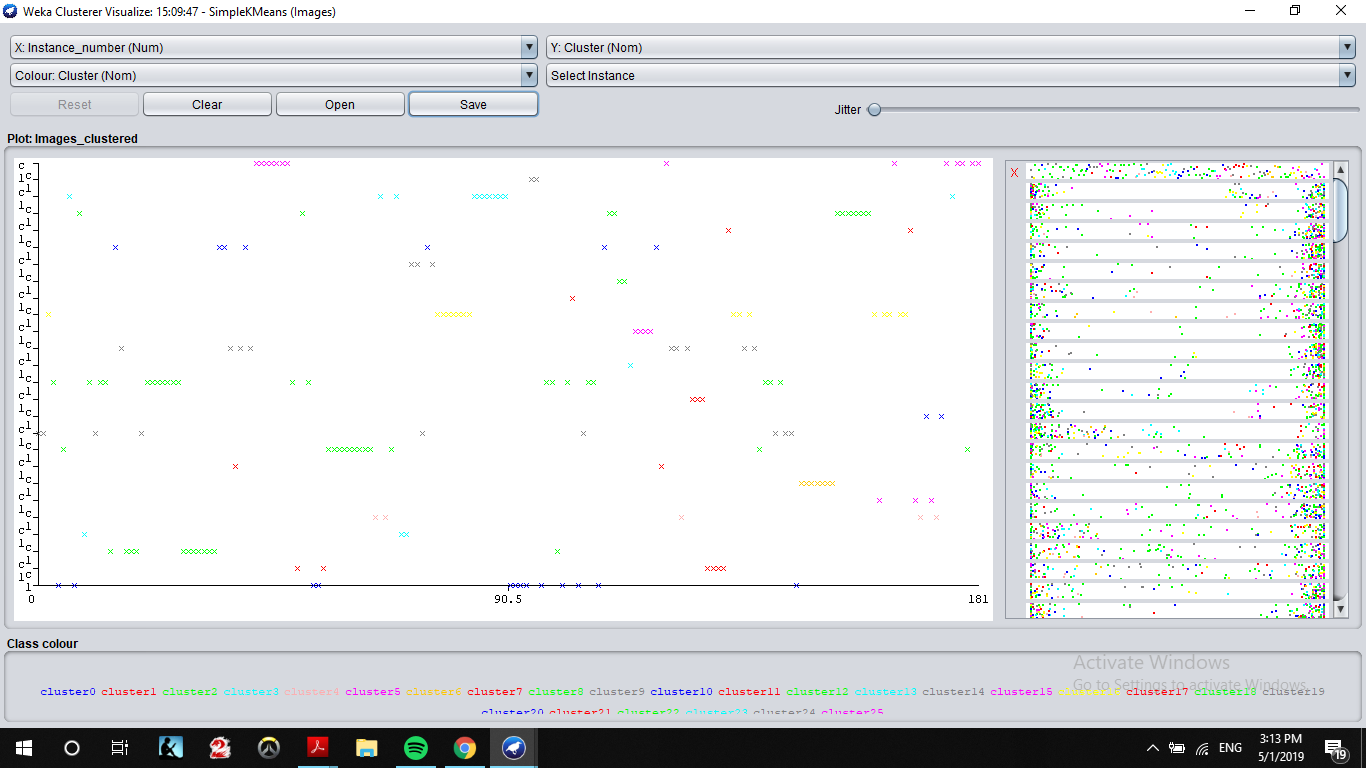
\includegraphics[width=1\textwidth]{kmeans.png}
	\caption{K-means clustering}
	\label{figure:kmeans}
\end{figure}

%----------------------------------------------------------------------------------------
%	Hierarchical Clustering with Single Linkage
%----------------------------------------------------------------------------------------
\newpage
\section{Hierarchical Clustering with Single Linkage}
\begin{table}[h!]
	\centering
	\caption{Results of clustering into 26 clusters}
	\label{table:single}
	\begin{tabular}{||c c c||} 
		\hline
		Cluster & No. Instances & Percentage \\ [0.5ex] 
		\hline\hline
		0 & 5 &  3\% \\
		1 & 2 &  1\% \\
		2 & 136 & 75\% \\
		3 & 1 & 1\% \\
		4 & 1 & 1\% \\
		5 & 1 & 1\% \\
		6 & 1 & 1\% \\
		7 & 1 & 1\% \\
		8 & 1 & 1\% \\
		9 & 1 & 1\% \\
		10 & 1 & 1\% \\
		11 & 7 & 4\% \\
		12 & 1 & 1\% \\
		13 & 1 & 1\% \\
		14 & 1 & 1\% \\
		15 & 1 & 1\% \\
		16 & 1 & 1\% \\
		17 & 6 & 3\% \\
		18 & 1 & 1\% \\
		19 & 1 & 1\% \\
		20 & 1 & 1\% \\
		21 & 1 & 1\% \\
		22 & 1 & 1\% \\
		23 & 5 & 3\% \\
		24 & 1 & 1\% \\
		25 & 1 & 1\%\\ [1ex] 
		\hline
	\end{tabular}
\end{table}
\newpage
\begin{figure}[h]
	\centering
	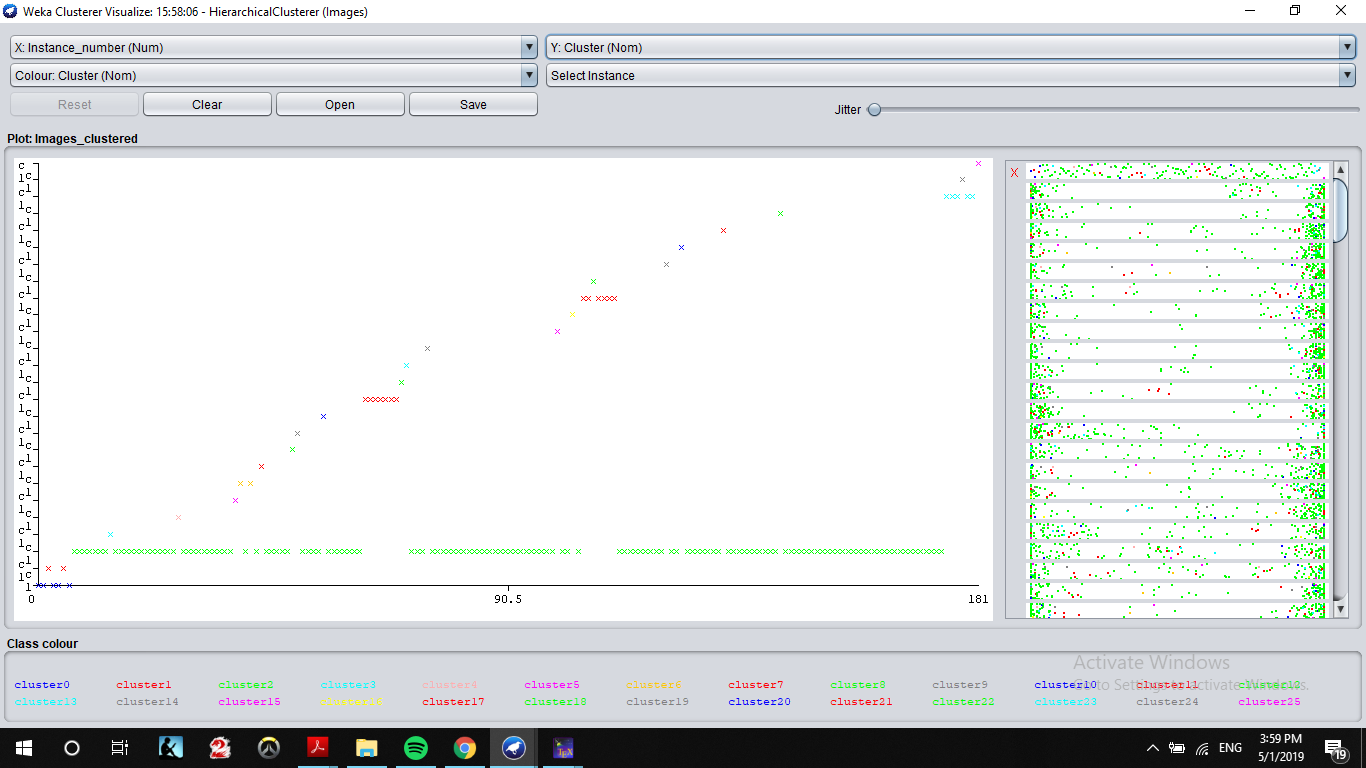
\includegraphics[width=1\textwidth]{single.png}
	\caption{Hierarchical Clustering with Single Linkage}
	\label{figure:single}
\end{figure}

%----------------------------------------------------------------------------------------
%	Hierarchical Clustering with Average Linkage
%----------------------------------------------------------------------------------------
\newpage
\section{Hierarchical Clustering with Average Linkage}
\begin{table}[h!]
	\centering
	\caption{Results of clustering into 26 clusters}
	\label{table:average}
	\begin{tabular}{||c c c||} 
		\hline
		Cluster & No. Instances & Percentage \\ [0.5ex] 
		\hline\hline
		0 & 7 &  4\% \\
		1 & 9 & 5\% \\
		2 & 7 & 4\% \\
		3 & 7 & 4\% \\
		4 & 9 & 5\% \\
		5 & 9 & 5\% \\
		6 & 1 & 1\% \\
		7 & 2 & 1\% \\
		8 & 7 & 4\% \\
		9 & 19 & 10\% \\
		10 & 9 & 5\% \\
		11 & 1 & 1\% \\
		12 & 21 & 12\% \\
		13 & 7 & 4\% \\
		14 & 6 & 3\% \\
		15 & 8 & 4\% \\
		16 & 1 & 1\% \\
		17 & 7 & 4\% \\
		18 & 7 & 4\% \\
		19 & 2 & 1\% \\
		20 & 6 & 3\% \\
		21 & 1 & 1\% \\
		22 & 1 & 1\% \\
		23 & 14 & 8\% \\
		24 & 7 & 4\% \\
		25 & 7 & 4\%\\ [1ex] 
		\hline
	\end{tabular}
\end{table}
\newpage
\begin{figure}[h]
	\centering
	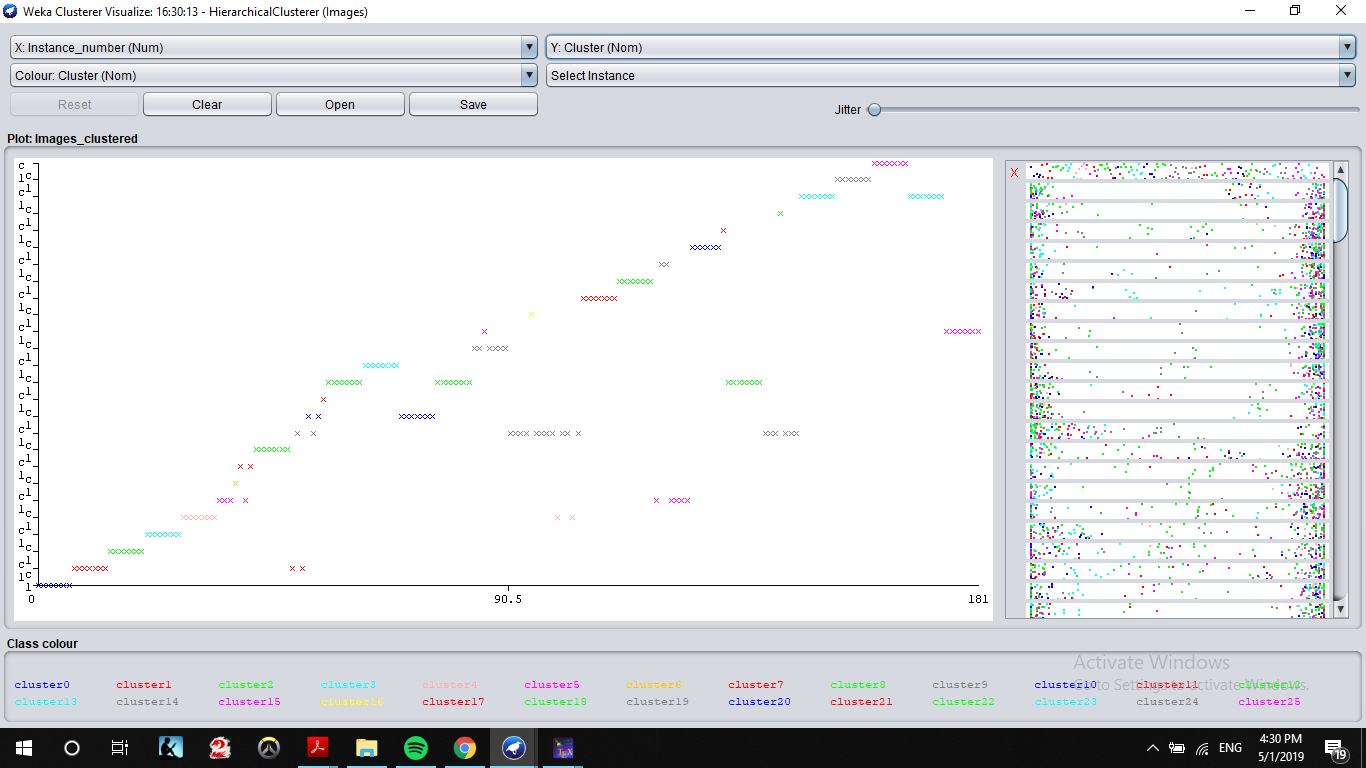
\includegraphics[width=1\textwidth]{average.png}
	\caption{Hierarchical Clustering with Average Linkage}
	\label{figure:average}
\end{figure}

%----------------------------------------------------------------------------------------
%	Hierarchical Clustering with Complete Linkage
%----------------------------------------------------------------------------------------
\newpage
\section{Hierarchical Clustering with Complete Linkage}
\begin{table}[h!]
	\centering
	\caption{Results of clustering into 26 clusters}
	\label{table:complete}
	\begin{tabular}{||c c c||} 
		\hline
		Cluster & No. Instances & Percentage \\ [0.5ex] 
		\hline\hline
		0 & 7 &  4\% \\
		1 & 7 & 4\% \\
		2 & 5 & 3\% \\
		3 & 7 & 4\% \\
		4 & 7 & 4\% \\
		5 & 9 & 5\% \\
		6 & 5 & 3\% \\
		7 & 6 & 3\% \\
		8 & 7 & 4\% \\
		9 & 5 & 3\% \\
		10 & 4 & 2\% \\
		11 & 5 & 3\% \\
		12 & 9 & 5\% \\
		13 & 7 & 4\% \\
		14 & 7 & 4\% \\
		15 & 12 & 7\% \\
		16 & 6 & 3\% \\
		17 & 8 & 4\% \\
		18 & 13 & 7\% \\
		19 & 7 & 4\% \\
		20 & 8 & 4\% \\
		21 & 2 & 1\% \\
		22 & 6 & 3\% \\
		23 & 2 & 1\% \\
		24 & 14 & 8\% \\
		25 & 7 & 4\%\\ [1ex] 
		\hline
	\end{tabular}
\end{table}
\newpage
\begin{figure}[h]
	\centering
	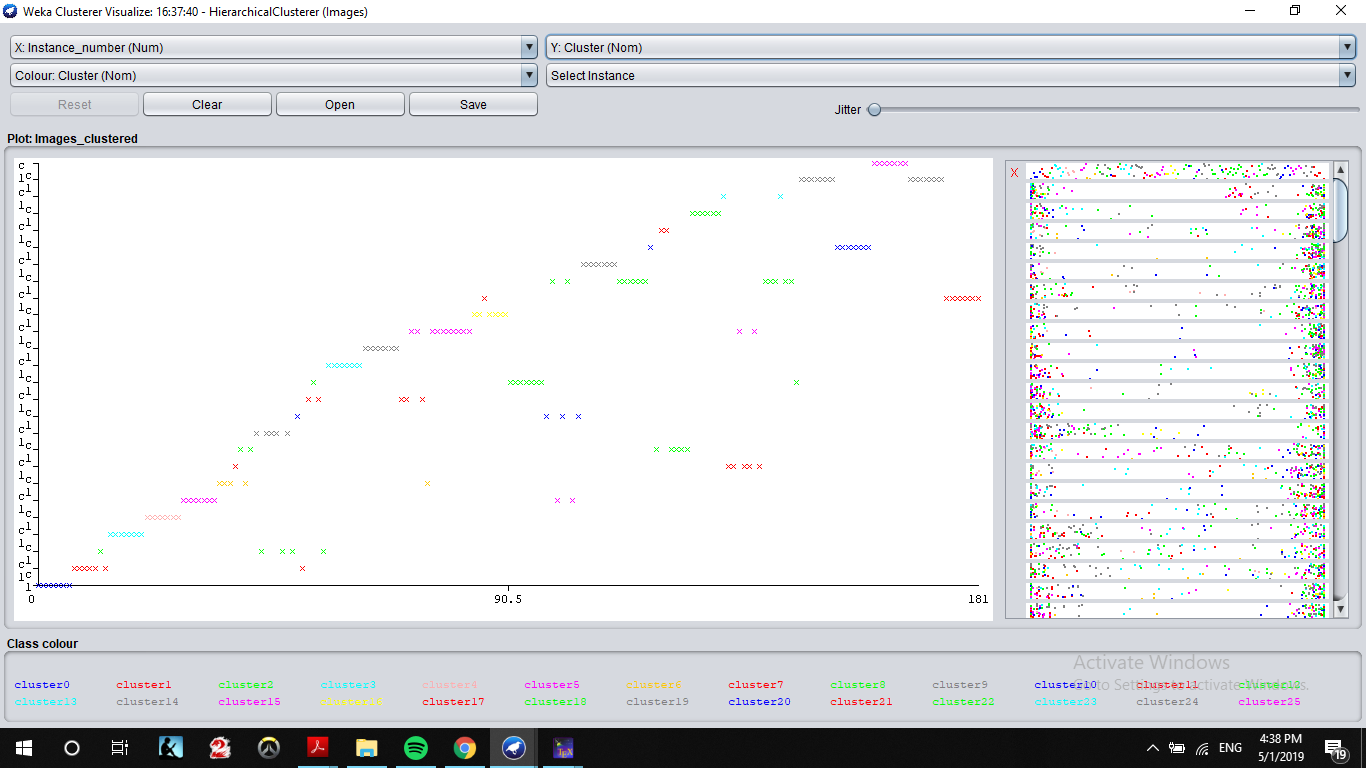
\includegraphics[width=1\textwidth]{complete.png}
	\caption{Hierarchical Clustering with Complete Linkage}
	\label{figure:complete}
\end{figure}

%----------------------------------------------------------------------------------------
%	Conclusion
%----------------------------------------------------------------------------------------
\newpage
\section{Conclusion}
Hierarchical clustering with single linkage performs worst of the four algorithms. As 136 (75\%) of the input gets assigned to a single cluster which should be only 7, as per table \ref{table:single} and figure \ref{figure:single}.

K-means clustering performed better than the hierarchical clustering with single linkage. However, a number of cluster contain only 1 or 2 instances, as per table \ref{table:kmeans} and figure \ref{figure:kmeans}.

Hierarchical clustering with average linkage and complete linkage provide similar clusters, to some extent. However, the number of misclassified instances is a bit less in complete linkage, by comparing table \ref{table:average}, figure \ref{figure:average}, table \ref{table:complete}, and figure \ref{figure:complete}. Meaning that hierarchical clustering with complete linkage provides the best results.

\end{document}